% xelatex -> biber -> xelatex*2
% chktex-file 1
% chktex-file 8
% chktex-file 9
% chktex-file 10
% chktex-file 17
% chktex-file 12
% chktex-file 18
% chktex-file 36
% chktex-file 38

\documentclass[12pt,twoside]{article}

\usepackage[a4paper,margin=1in]{geometry}
\usepackage{setspace}
\usepackage{fontspec}
\setmainfont{Times New Roman}
\usepackage{enumitem}
\usepackage[hidelinks]{hyperref}
\usepackage{xcolor}
%\usepackage{ragged2e}

\usepackage{graphicx}
\usepackage{caption}
\captionsetup{labelfont=bf,font=footnotesize}

% single spaced, blank line between paragraphs
\setlength{\parindent}{0pt}
\setlength{\parskip}{\baselineskip}
\setstretch{1}

% Keep interword spacing uniform (avoid stretched spaces from full justification)
%\RaggedRight

% ---- APA 7 references with biblatex ----
\usepackage[
  backend=biber,
  style=apa,
  sorting=nyt
]{biblatex}
\DeclareLanguageMapping{english}{english-apa}
\addbibresource{references.bib}

\defbibheading{normalrefs}[\bibname]{%
  \setlength{\parskip}{0pt}% no extra blank line after heading
  \textbf{#1}\par
}

\usepackage[draft]{changes} % use 'draft' instead of 'final' to see changes
\definechangesauthor[name={YizhanFeng}, color=red]{G}
\definechangesauthor[name={YizhanFeng}, color=purple]{W}
\setauthormarkup{}

\usepackage{fancyhdr}
\pagestyle{fancy}
\fancyhf{} % clear all header/footer fields

% Optional: no header rule line
\renewcommand{\headrulewidth}{0pt}

% Make sure header has enough height for two lines
\setlength{\headheight}{26pt}

% Odd-page header, top left, gray text
\fancyhead[LO]{\small\textcolor{gray}{CTAW (Zhang)\\2025 Fall}}

% Footers: [page number] | [Title]. Odd pages: bottom left; Even pages: bottom right
\fancyfoot[LO]{\footnotesize\textcolor{gray}{\thepage\ \textbar\ ``Us'' v.s. ``Them'' in 1080p: Partisan Meme Wars During the 2024 U.S. Election}}
\fancyfoot[RE]{\footnotesize\textcolor{gray}{\thepage\ \textbar\ ``Us'' v.s. ``Them'' in 1080p: Partisan Meme Wars During the 2024 U.S. Election}}


\begin{document}

{\fontsize{16}{35}\selectfont
Critical Thinking \& Academic Writing\\
Project paper\par
}

\vspace{-0.5\baselineskip}

Class: C5 \\
Name: Yizhan Feng \\
Draft: D4 (2025.12.30) \\

\vspace{-0.75\baselineskip}

\begin{center}
{\fontsize{14}{17}\selectfont
``Us'' v.s. ``Them'' in 1080p: Partisan Meme Wars During the 2024 U.S. Election\par
}
\end{center}

\vspace{-\baselineskip}

% 1. Introduction

For many young Americans, the 2024 U.S. presidential election was experienced less through televised debates or newspaper columns and more through short videos and images on TikTok and X. Surveys by the Pew Research Center show that by 2024, about one-third of adults aged 18 to 29 regularly got their news from TikTok, with significant shares also using X and Instagram for political information \parencite{shearer2024newsTikTokXFacebookInstagram}. Within these platforms, memes---humorous images, short videos, and text formats that are rapidly remixed and shared \parencite[39]{shifman2013memesdigitalculture}---became a central medium for expressing political views. Media outlets compiled lists of ``the memes that defined the 2024 election season'', underscoring how\deleted{ meme streams}\added{ viral jokes} shaped many young voters’ sense of the campaign.

However, many of these memes were not neutral jokes; they were partisan weapons, crafted and spread by supporters of each camp to hype their own side and mock the other. How do partisan memes on the Internet construct ``us'' and ``them'' in the 2024 U.S. election, and how is engagement with partisan meme warfare related to young users' sense of partisan identity and their willingness to interact with people from the opposing party? In light of these questions, this paper argues that partisan memes frame electoral politics as an antagonistic relationship between a virtuous, relatable ``us'' and a corrupt\deleted{ or}\added{,} ridiculous ``them''. Among young users,\deleted{ heavy}\added{ extensive} engagement with partisan meme content is associated with stronger partisan identity and lower openness to cross-party interaction, thereby contributing to affective polarization. To ground these arguments, the following section will review key scholarship on memes, trace their role in recent U.S. elections, examine how they are weaponized and connect their circulation to broader patterns of affective polarization.

% 2. Literature Review

Although Internet users have only widely encountered ``meme'' in recent decades, the term itself was conceived long before the digital era.\deleted{The term \textit{meme}, c}\added{ C}oined by \textcite{dawkins1976selfishgene},\added{ it} originally described small cultural units that spread by imitation. In the Web 2.0 era, \textcite{shifman2013memesdigitalculture} redefined Internet memes as characterized by creative production and intertextuality: users constantly adapt and remix templates while weaving together multiple cultural references and contexts. \textcite{shifman2013memesdigitalworld} further explored a three-dimensional typological framework for memetic analysis that breaks memes down into ``content, form, and stance''. In partisan meme wars, the creative production and intertextuality of memes largely operate on the levels of content and form, while stance functions as the crucial ``switch'' that tells in-group audiences how to feel and where the line between ``us'' and ``them'' should be drawn.

Compared with other online symbols such as straightforward text posts or static campaign logos, Internet memes are thus distinctive in how efficiently they carry stance. Their humor, remixability, and dense intertextuality make them attractive to platform algorithms that reward engagement, while their playful ambiguity offers plausible deniability (``it's just a joke'') even when they carry strongly biased messages \parencite{yoon2016notjustajoke}. Sharing a meme becomes a low-cost identity performance: by reposting a familiar template or clip, users publicly signal which side they belong to and which side they ridicule.
 
% 3. Memetic Weaponization

\begin{figure}[htbp]
  \centering
  \begin{minipage}[t]{0.48\textwidth}
    \centering
    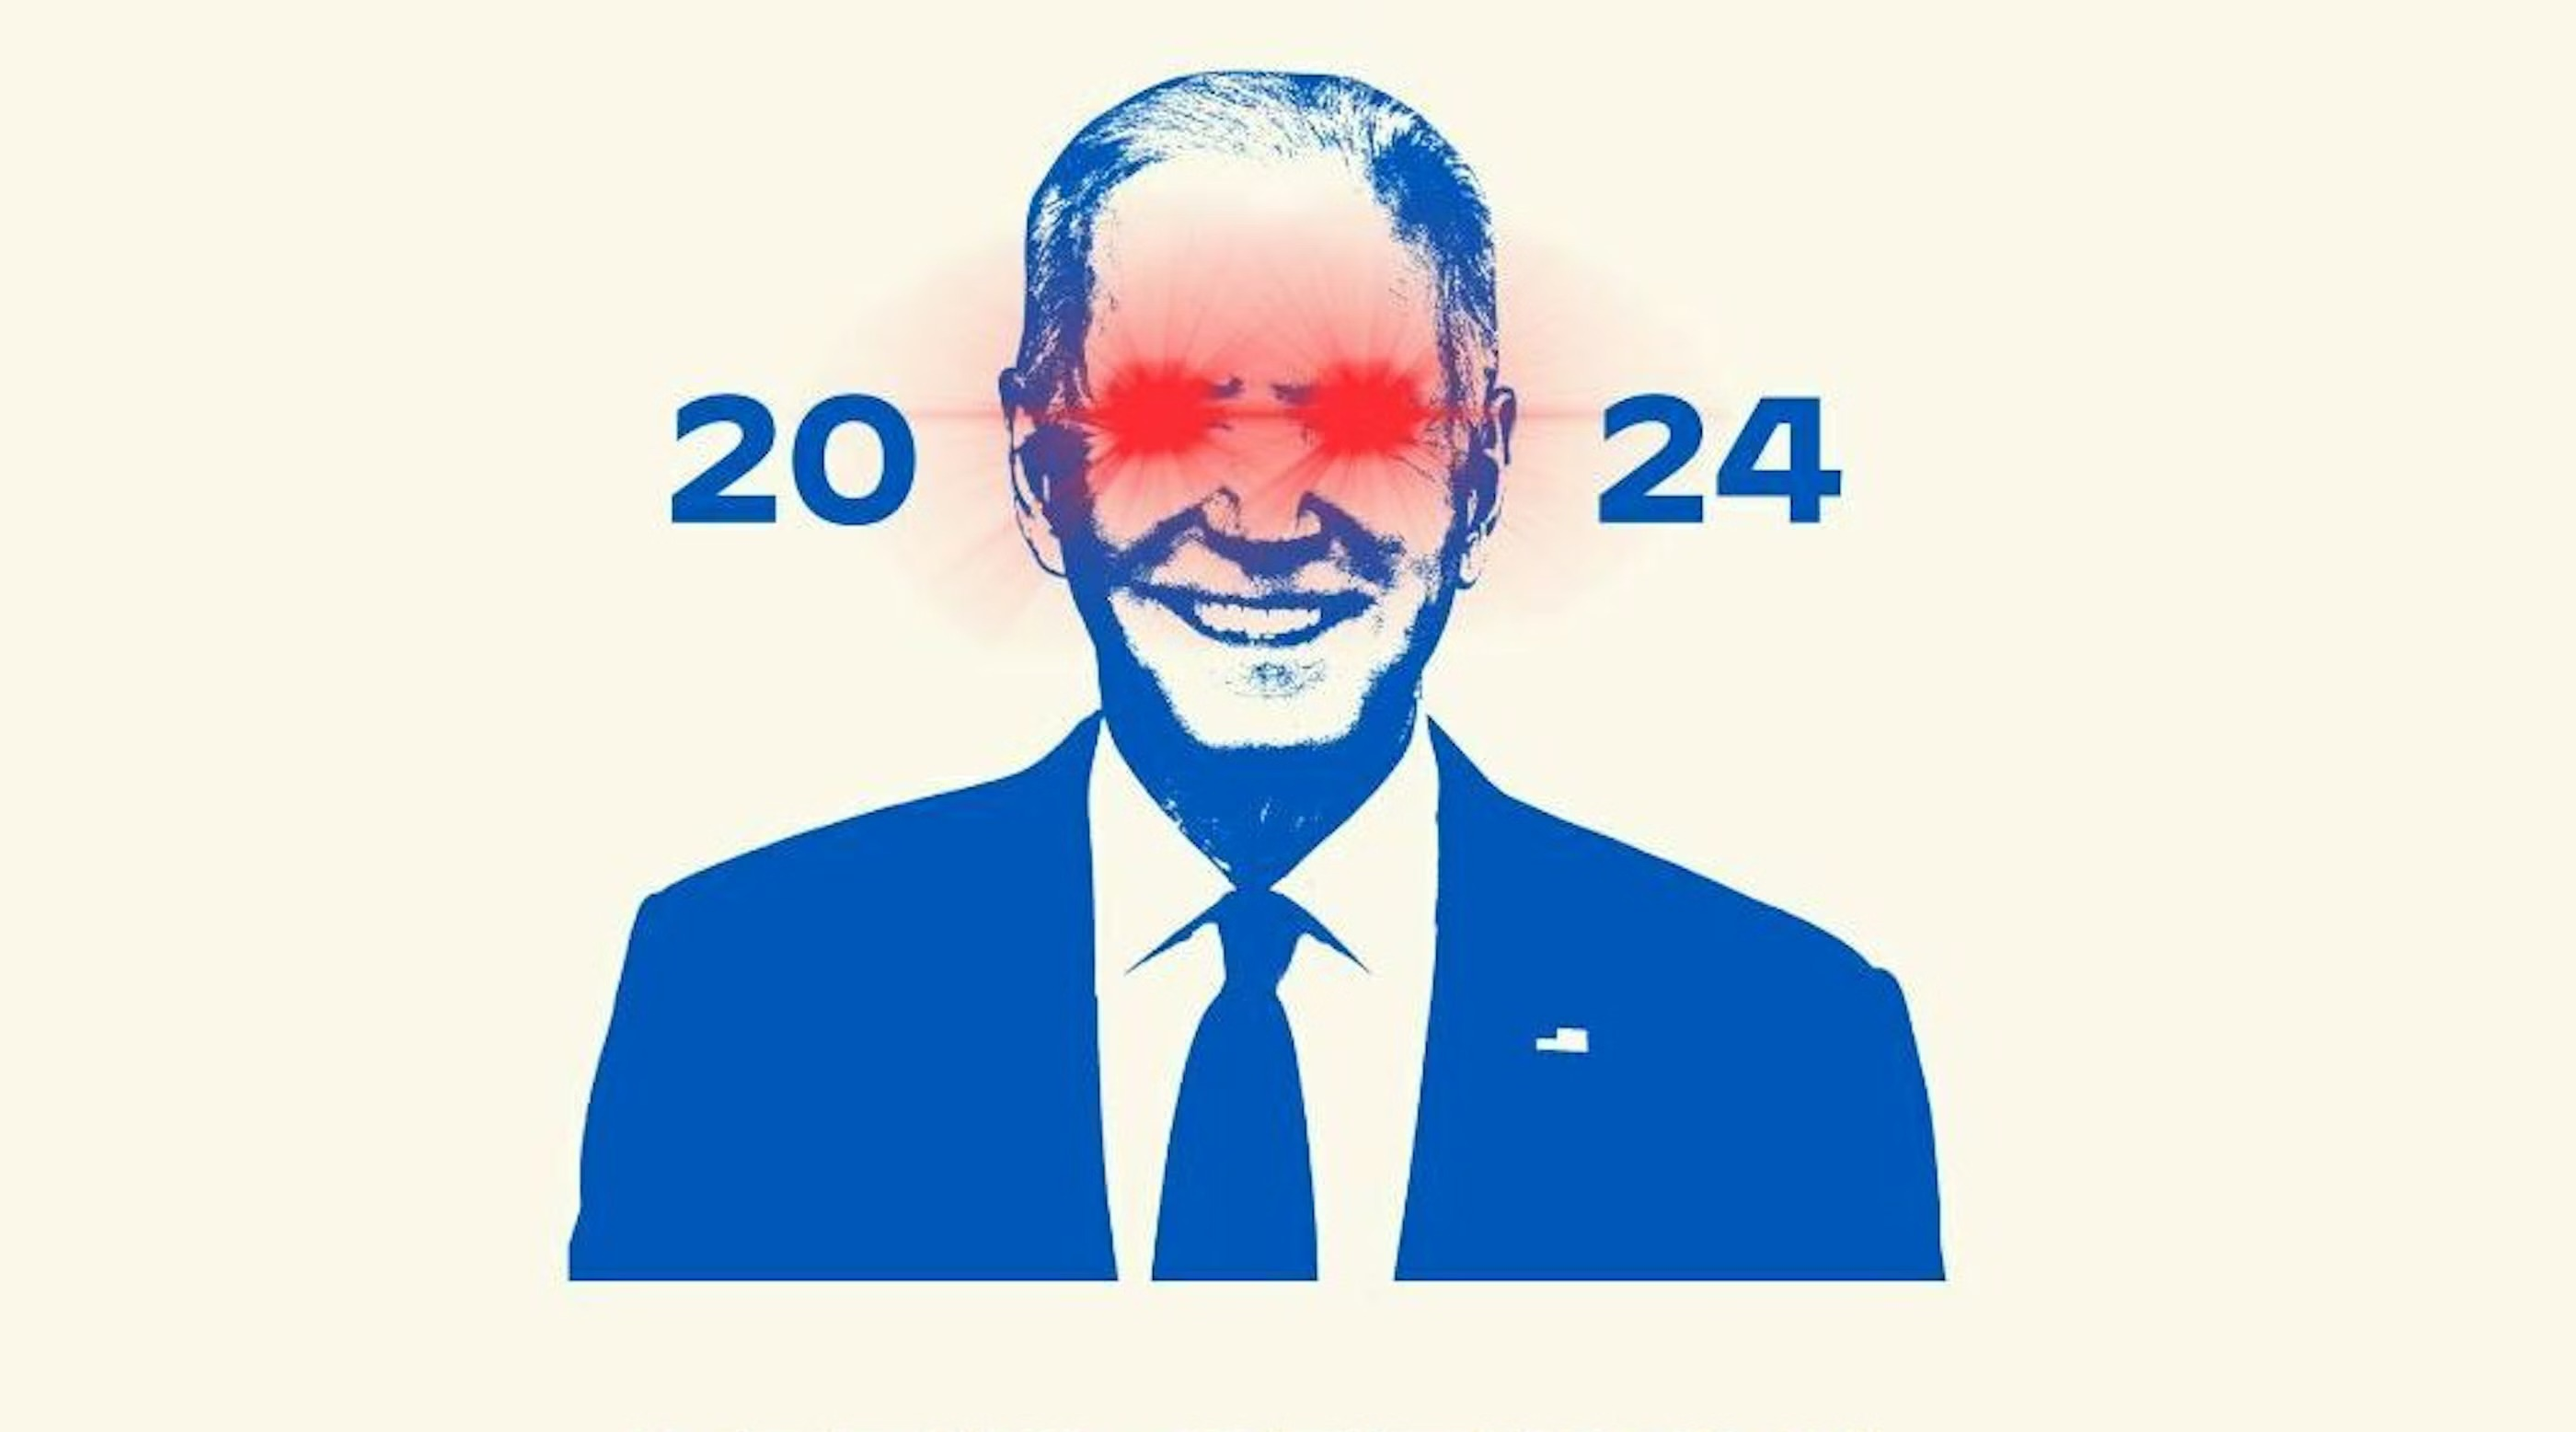
\includegraphics[width=\linewidth]{Figures/DarkBrandon.jpg}
    \caption{Biden's ``Dark Brandon'' meme}
  \end{minipage}\hfill
  \begin{minipage}[t]{0.48\textwidth}
    \centering
    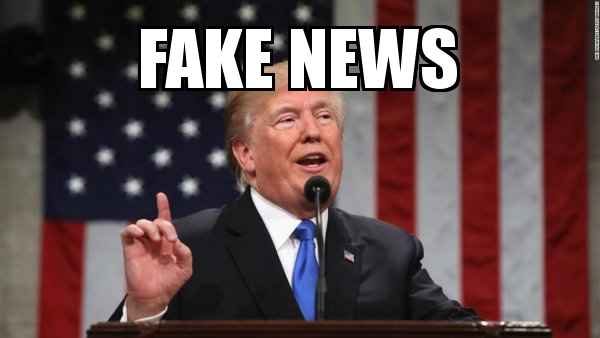
\includegraphics[width=\linewidth]{Figures/FakeNews.jpg}
    \caption{Trump's ``Fake News'' meme}
  \end{minipage}
\end{figure}

Against this backdrop, Internet memes have played an increasingly visible role in recent U.S. presidential elections. Since 2016, supporters have used memes on platforms such as Facebook and Reddit to circulate grassroots political messages, normalize pro-candidate narratives, and attack opponents through irony and ridicule \parencite{hunting2020popularmediamemes, moodyramirez2019facebookmemegroups}. By 2024, meme logics were no longer confined to fringe communities: major campaigns actively leaned into viral formats, as the Biden-Harris team did when it embraced the ``Dark Brandon'' meme\deleted{ and laser-eyed images of the president} across TikTok and X\deleted{, recasting him}\added{ to recast the president} as an almost superheroic guardian of ``our'' side\deleted{ and}\added{,} signaling ironic strength and insider humor to young supporters \parencite{robertson2024bidenmemelord,mielczarek2024darkbrandonenthymeme}. On the Republican side, Donald Trump's catchphrase ``Fake News'' itself had been repeatedly used not only as a meme template but also as a form of ``weaponized iconoclastic multimodal propaganda'' \parencite[303]{smith2019weaponizediconoclasm} to portray Trump himself as the only truthful voice and construct a moral divide between a betrayed ``people'' and a corrupt ``establishment'' \parencite{ross2018discursivedeflection,woodward2020fakenewsguide}. Rather than replacing traditional campaign communication, these partisan meme streams now run alongside official messaging, offering highly shareable visual narratives that help each side define its heroes, villains, and version of what is at stake in the election.

However, these memes were not neutral artifacts that\deleted{ simply popped up from nowhere and} went viral randomly. Rather, they were deliberately selected and circulated as ``discursive weapons'' to ``justify judgement, condemnation, and exclusion of others'' \parencite[495]{nissenbaum2017contestedculturalcapital}. \textcite[218-219]{peters2021weaponizingmemes} proposed this concept of memetic weaponization as ``purposeful deployment of memetic imagery to disrupt, undermine, attack, resist, or reappropriate discursive positions about public affairs in and around the news''. By serving as ``identificatory markers of affiliation'' \parencite[219]{peters2021weaponizingmemes}, these memes successfully hijacked netizens' attention for political propaganda \parencite{olsen2018weaponizedmemes} and advanced a politics of othering, signaling who counts as in-group and who does not.\deleted{ Taken together, t}\added{ T}hese examples show how, by the 2024 election, both parties had weaponized memes as low-cost, high-effect tools for drawing the line between a morally superior, relatable ``us'' and an incompetent, dangerous ``them''. 

% 4. ``Coconut tree'' Case Analysis

\begin{figure}[htbp]
  \centering
  \begin{minipage}[t]{0.48\textwidth}
    \centering
    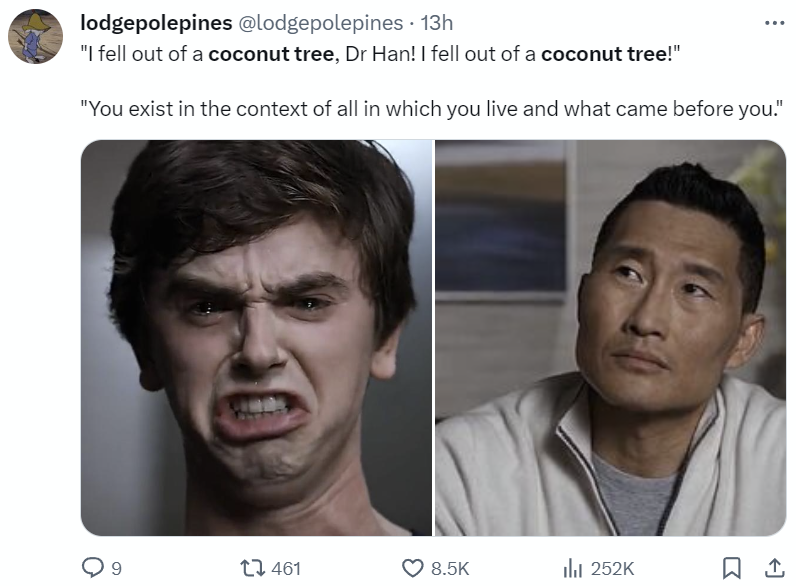
\includegraphics[width=\linewidth]{Figures/RepublicanCTM.png}
    \caption{Republican-aligned ``Coconut Tree'' meme}
  \end{minipage}\hfill
  \begin{minipage}[t]{0.48\textwidth}
    \centering
    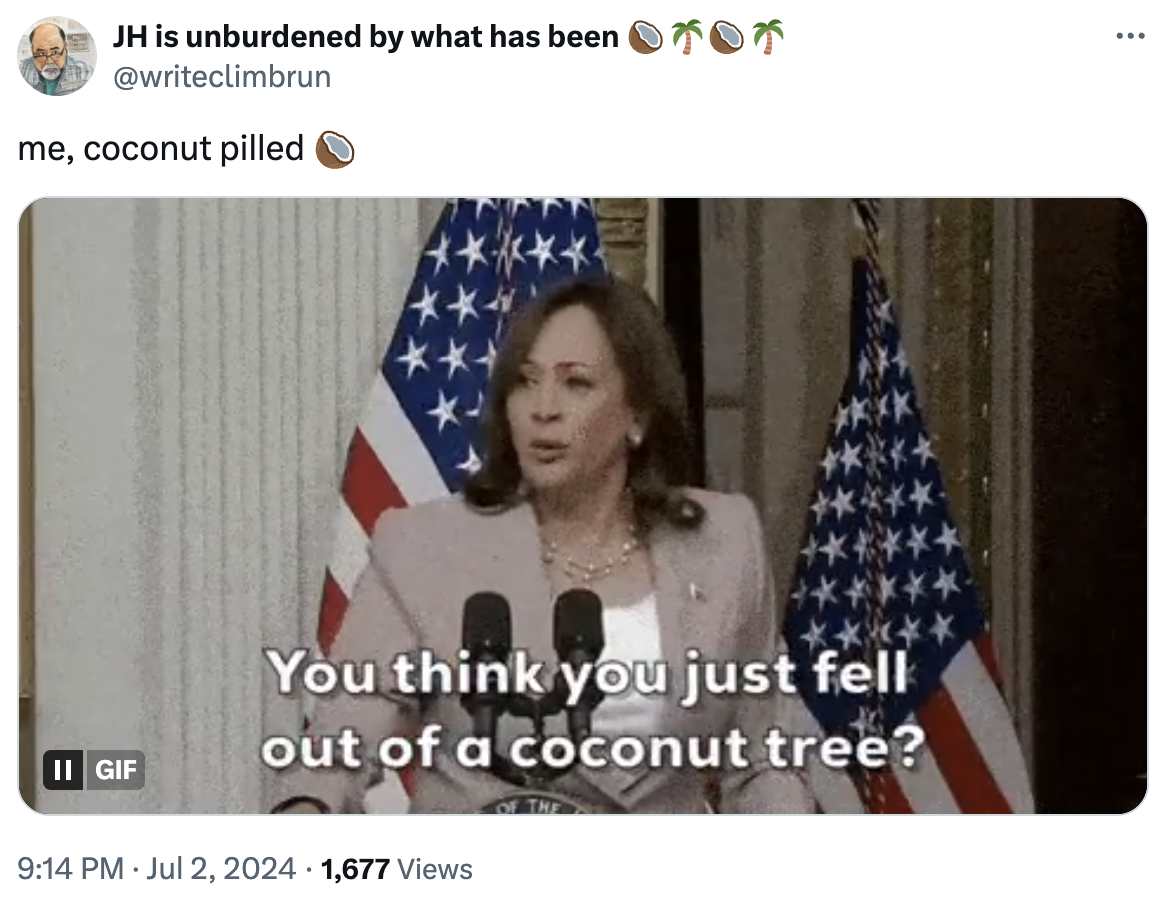
\includegraphics[width=\linewidth]{Figures/DemocratCTM.png}
    \caption{Democrat-aligned ``Coconut Tree'' meme}
  \end{minipage}
\end{figure}

One emblematic dynamic in this memetic warfare is the ``coconut tree'' meme around Kamala Harris. The meme originated from a May 10, 2023 White House speech, where Harris quoted her mother: ``You think you just fell out of a coconut tree?'', meaning that young people are shaped by families, communities, and history rather than existing ``in a silo'' \parencite{harris2023swearinginremarks}. This memefied fragment of Harris's speech was initially circulated by conservative Republican-aligned accounts as a vehicle of mockery, presenting Harris as incoherent, incomprehensible and fundamentally incapable\deleted{. This strategy was effective, as the dominant reading on X was that Harris was}\added{; on X, the dominant reading framed her as} ``weird'' or ``blissfully insane'', with users pairing the audio with reaction images to ridicule her \parencite{carry2024coconuttreeguide}. However, as Biden's position weakened, young Democrats online rallied to Harris and flipped the meme: coconut and palm-tree emojis in bios and display names became a shorthand for backing Harris \parencite{coleman2024coconutmeme}, and supporters jokingly called themselves ``coconut-pilled'', adapting right-wing ``red-pilled'' language to signal\deleted{ that they had enthusiastically converted}\added{ an enthusiastic conversion} Harris fandom \parencite{roberts2024coconuttreeorganic}.

\deleted{This example is a robust validation}\added{ This trajectory offers a vivid illustration} of \textcite{shifman2013memesdigitalculture}'s memetic framework.  While the meme's content and form remained largely unchanged, a simple shift in stance---from ``she's cringe, unserious, not presidential'' to ``she's a little weird, but in a fun, relatable, mom-wisdom way—and she's \textit{our} candidate''---allowed the same coconut tree clip to perform radically different discursive functions. Republicans weaponized the meme as an out-group attack focused on mockery and delegitimization, labeling ``them'' (Harris and the Democrats) as bizarre and unfit. Democrats, on the other hand, embraced this hostile meme and reframed the quote as an empowering in-group hype, drawing a clear boundary between the playful, self-aware, community-rooted ``us'' and the unrelatable ``them'' who fail to understand the context. In this way, shifts in stance do not just change the surface meaning of a meme; they restructure the social relationships that the meme organizes, intensifying the ``us''/``them'' dynamic within online communities.

% 5. Affective Polarization

Taken together, these examples suggest that partisan meme warfare is increasingly blurring the line between entertainment and political participation. While scholars have documented the positive effect of political memes in opening up new participatory gateways for political engagement from below \parencite{sreekumar2013onlinepoliticalmemes, ahmed2024breakingbarriersmemes, mushtaq2025betweenhumorharm}, others warn that such participatory gains come with important \deleted{affective} costs, namely affective polarization. Following \textcites[405]{iyengar2012affectnotideology}[691]{iyengar2015fearloathing}[130]{iyengar2019originsaffectivepolarization},\deleted{ affective polarization}\added{ it} is defined as the growing tendency for partisans to evaluate their own side warmly while feeling dislike, distrust, and even disgust toward supporters of the opposing party. Rather than being driven \deleted{purely} by ideological distance, this form of polarization flows from social identity dynamics: seeing oneself as a loyal Democrat or Republican becomes a powerful basis for in-group favoritism and out-group animus.  

The 2024 election meme wars are likely to intensify this tendency. Quantitative analyses of mainstream political memes across recent U.S. election cycles show that the most heavily shared memes are strongly partisan in both content and stance, portraying the out-party as stupid, hypocritical, or dangerous while casting the in-party as sensible and morally righteous \parencite{collier2024compositionmainstreammemes}. As \textcite[1]{alafnan2025roleMemesPoliticalDiscourse} notes, political memes ``serve as instruments for reinforcing ideological divides''. Rather than showing political opponents as ordinary citizens with different priorities, memes most often depict them as laughable or threatening caricatures, making the ``other side'' feel less legitimate and less human. By providing short runtimes and small canvases that encourage binary moral narratives, meme formats cloak hostility in humor and bake ``us\deleted{ vs}\added{ v.s.} them'' logics into their very form, further reinforcing the echo chamber effect. \textcite{kim2023partisanmemes}'s network studies confirm that engaging with partisan memes tends to catalyze homophilous online networks, as users who like or share such memes increasingly interact with like-minded others and see less cross-cutting content, reinforcing an ``us v.s. them'' structure in their feeds.\deleted{ Experimental work suggests that exposure to out-group-targeting memes does not so much persuade people to change sides as it entrenches existing identities, increasing polarization especially among strong partisans \parencite{galipeau2023impactpoliticalmemes}.} Combined with platform algorithms that reward emotionally intense, in-group-affirming content \parencite{ye2025auditingexposurebias}, these dynamics mean that the same meme practices which draw young voters into politics also socialize them into experiencing politics as a zero-sum struggle against a contemptible ``them''---precisely the emotional pattern captured by the concept of affective polarization.

% 6.Counterargument

Still, it is important not to overstate the negative impact of partisan meme wars. Memes do not operate in a vacuum: they appear embedded in captions, comment sections, and recommendation feeds that shape how audiences interpret them. The same coconut tree clip, for instance, might be posted in an explicitly political thread with a caption attacking Harris, but it might also circulate in more casual ``cringe compilation'' or fan-edit contexts where the focus is on entertainment rather than electoral choice. Young users can encounter the same image macro as a serious political statement in one context and as a silly in-joke in another.

Moreover, the young people most active in producing and sharing partisan memes may already be highly engaged and strongly identified with a party. For them, meme warfare probably does not flip their loyalties; instead, it solidifies pre-existing identities, giving them emotionally satisfying ways to celebrate ``us'' and condemn ``them'' \parencite{galipeau2023impactpoliticalmemes}. A teenager who occasionally encounters a Trump ``Fake News'' meme in a non-political group chat might chuckle and scroll on, while a committed partisan in a politicized TikTok bubble may interpret the same image as a rallying symbol or an unforgivable insult. From this perspective, partisan memes might function less as tools of mass persuasion and more as mechanisms for maintaining already polarized communities.\deleted{ They solidify pre-existing identities, rather than flipping loyalties.}

% 7.Conclusion

Overall, partisan meme wars are double-edged: they energize and mobilize young voters, provide an outlet for anxiety and creativity, and help people feel that they are part of something larger. At the same time, they flatten complex issues into jokes and enemies, rewarding those who shout the loudest and mock the hardest. For democratic discourse, this raises a difficult question: how can societies harness the participatory power of memes without letting politics devolve into endless digital trench warfare? Answering this question requires not only platform governance and campaign ethics but also everyday critical literacy. Recognizing memes as simultaneously invitations to belong and cues to distrust may encourage young citizens, when they scroll past yet another Trump meme or coconut-tree clip, to pause before liking and reposting it and to ask instead what kind of ``us'' and ``them'' the meme is inviting them to imagine.


\vspace{-\baselineskip}

\begin{flushright}\textbf{(1914 words)}\end{flushright}

\vspace{-\baselineskip}

\textbf{Declaration of generative AI and AI-assisted technologies in the writing process.}\\
During the preparation of this work, I used ChatGPT in order to\deleted{ brainstorm topics, summarize literature and generate title and revision suggestions}\added{ help brainstorm possible angles for narrowing my topic, to assist me in identifying key themes in readings, and to offer alternative titles and revision suggestions (e.g., improving clarity and structure)}. After using this tool/service, I reviewed and edited the content as needed and take(s) full responsibility for the content of the submitted project paper.
\deleted{[Your reflection]}\added{I learned to be cautious about over-relying on AI, not treating its outputs as authoritative. Any literature summaries were checked against the original sources, and I verified wording, concepts, and citations myself. I also revised the AI-generated suggestions substantially to match my own argument, evidence, and writing style. I am aware that generative AI can produce incomplete or inaccurate information, so I used it only to support idea development and editing, not to replace my own reading, analysis, or responsibility for the final content.}

\vspace{\baselineskip}

\printbibliography[heading=normalrefs,title={References}]

\end{document}